\documentclass[11pt]{article}
\newcommand{\oa}{\overline{a}}
\newcommand{\ob}{\overline{b}}
\newcommand{\oc}{\overline{c}}
\newcommand{\oi}{\overline{i}}

\newcommand{\integermodn}[1][n]{\Z/#1\Z}
\newcommand{\integermodnmul}[1][n]{(\Z/#1\Z)^{\times}}
\newcommand{\order}[1]{\left|#1\right|}
\newcommand{\modb}[1]{\left(mod \;\; #1 \right)}
\newcommand{\aut}[1]{Aut\left(#1\right)}
\newcommand{\actson}{\ensuremath{\curvearrowright}}

\newcommand{\heading}[1]{(#1)}
\newcommand{\bheading}[1]{\textbf{(#1)}}

% arg1=pdfurl arg2=pagenum arg3=text
\usepackage{url}
\usepackage{hyperref}
\hypersetup{colorlinks=true, linktoc=all, linkcolor=blue}
\newcommand{\linkbook}[3][../../abstract_algebra_dummit_and_foote.pdf]{
    \noindent\href[page=#2]{#1}{\urlstyle{rm}{#3}}
}

\usepackage[a4paper, total={6in, 8in}, margin=0.5in]{geometry}

\usepackage{listings}
\usepackage{hyperref}
\graphicspath{{assets/}}

\title{CSC446 A2}
\author{Peiqi Wang 1001132561}


\begin{document}

\maketitle
    
\section*{Problem 1 (chapter 9 q9.2)}
Find explicitly the coefficients $a_{k,l}$ where $k,l=1,2,\cdots,m$ for 
\[
    -y'' + y = f    
\]
assuming the space $\mathbb{H}^{\circ}_m$ is spanned by the chapeau function on an equidistant grid
\begin{proof}
    This is a special case of the ODE we discussed in class. We get the expression for $a_{k,l}$ as
    \[
        a_{k,l} 
        = \inner{\varphi_l'(x)}{\varphi_k'(x)} + \inner{\varphi_l(x)}{\varphi_k(x)}
        = \int_0^1 \varphi_l'(x) \varphi_k'(x) dx + \int_0^1 \varphi_l(x) \varphi_k(x) dx
    \]
    where $\varphi_k(x)$ is given by the chapeau function 
    \[
        \varphi_k(x) = 
        \begin{cases}
            1 - k + \frac{x}{h} & (k-1)h \leq x \leq kh \\
            1 + k - \frac{x}{h} & kh \leq x \leq (k+1)h \\
            0 & \abs{x-kh} \geq h
        \end{cases}  
    \]
    $a_{k,l} \neq 0$ if and only if $\abs{k-l} < 2$. Now we do integration and compute $a_{k,k-1}, a_{k,k}, a_{k,k+1}$ 
    \begin{align*}
        a_{k,k+1} 
        &= \int_{kh}^{(k+1)h} \pc{
            -\frac{1}{h} \frac{1}{h} + 
            \p{1+k-\frac{x}{h}} \p{-k+\frac{x}{h}}
        } dx
        = \frac{h^2-6}{6h} \\
        a_{k,k}
        &= \int_{(k-1)h}^{kh} \pc{
            \frac{1}{h} \frac{1}{h} + 
            \p{1-k+\frac{x}{h}}^2
        } dx
        + \int_{kh}^{(k+1)h} \pc{
            \frac{1}{h} \frac{1}{h} + 
            \p{1+k-\frac{x}{h}}^2
        } dx
        = \frac{2(h^2+3)}{3h} \\
        a_{k,k-1}
        &= \int_{(k-1)h}^{kh} \pc{
            -\frac{1}{h} \frac{1}{h} + 
            \p{k-\frac{x}{h}} \p{1-k+\frac{x}{h}}
        } dx
        = \frac{h^2-6}{6h}
    \end{align*}
    with the help of online integral calculator. Therefore 
    \[
        a_{k,l} = 
        \begin{cases}
            \frac{2(h^2+3)}{3h} & l = k \\
            \frac{h^2-6}{6h} & l = k-1,k+1 \\
            0 & \text{otherwise} \\
        \end{cases} 
    \]
\end{proof}
 

\newpage
\section*{Problem 2 (chapter 9 q9.3)}
Suppose equation (9.1) 
\[
    - \frac{d}{dx} \pb{
        a(x) \frac{du}{dx}
    } + b(x)u = f
\]
is solved by Galerkin method with chapeau functions on a non-equidistant grid. In other words, we are given $0=t_0<t_1<\cdots < t_m<t_{m+1} = 1$ such that each $\varphi_k$ is supported in $(t_{k-1}, t_{k+1})$ for $k=1,2,\cdots,m$. Prove that the linear system (9.7) 
\[
    \sum_{l=1}^m a_{k,l} \gamma_l = \int_0^1 f(\tau) \varphi_k(\tau) d\tau - a_{k,0} \quad \quad k=1,2,\cdots,m    
\]
where 
\[
    a_{k,l} = \int_0^1 \pb{
        a(\tau) \varphi'_l(\tau) \varphi'_k(\tau) + b(\tau) \varphi_l(\tau) \varphi_k(\tau)
    } d\tau
\]
is nonsingular (Hint: Use Gersgorin criterion). State any additional assumptions that you need to ensure that the system is nonsingular.
\begin{proof}
    Idea is to show that 0 is not inside any Gersgorin disk. Consider expression for $\mathbb{S}_k$
    \begin{align*}
        \mathbb{S}_k = \pc{
            c \in \C \mid \abs{z - a_{k,k}} \leq \abs{a_{k,k-1} + a_{k,k+1}}
        }
    \end{align*}
    It is trivial to show that $a_{k,k-1},a_{k,k+1}$ have the same sign; so it is OK to right 1 absolute sign on right hand side. Now we write formula for the hat function 
    \[
        \varphi_k(x) = 
        \begin{cases}
            \frac{x-t_{k-1}}{t_k - t_{k-1}} & t \in [t_{k-1}, t_k] \\
            \frac{t_{k+1} - x}{t_{k+1} - t_k} & t \in [t_k, t_{k+1}] \\
            0 & \text{otherwise} \\
        \end{cases}    
    \]
    To show that 0 not in any $\mathbb{S}_k$, consider the region $[t_{k-1},t_k]$ which supports $\varphi_{k-1}(x)$ and $\varphi_k(x)$ but not $\varphi_{k+1}(x)$. So suffice to show $a_{k,k} > \abs{a_{k,k-1}}$, i.e. $a_{k,k} + a_{k,k-1} > 0$ and $a_{k,k} - a_{k,k-1} > 0$
    \begin{align*}
        a_{k,k} + a_{k,k-1}
        &= \int_{t_{k-1}}^{t_k} a(x) \p{\frac{1}{t_k - t_{k-1}}}^2 + b(x) \p{\frac{x-t_{k-1}}{t_k - t_{k-1}}}^2 dx \\
        &+ \int_{t_{k-1}}^{t_k} a(x) \p{-\frac{1}{t_k-t_{k-1}}}\p{\frac{1}{t_k - t_{k-1}}} + b(x) \p{\frac{t_k-x}{t_k-t_{k-1}}} \p{ \frac{x-t_{k-1}}{t_k - t_{k-1}} } dx \\
        &= \int_{t_{k-1}}^{t_k} b(x) \frac{1}{(t_k-t_{k-1})^2} \pc{
            (x-t_{k-1})^2 + (t_k-x)(x-t_{k-1})
        } dx \\ 
        &= \int_{t_{k-1}}^{t_k} b(x) \frac{t_k-t_{k-1}}{(t_k-t_{k-1})^2} \pc{x - t_{k-1}} dx
    \end{align*}
    which is greater than zero, since $b(x) \geq 0$ and $x-t_{k-1} \geq 0$ on $x\in [t_{k-1}, t_k]$. Now consider
    \begin{align*}
        a_{k,k}-a_{k,k-1}
        &= \int_{t_{k-1}}^{t_k} a(x) \p{\frac{1}{t_k - t_{k-1}}}^2 + b(x) \p{\frac{x-t_{k-1}}{t_k - t_{k-1}}}^2 dx \\
        &- \int_{t_{k-1}}^{t_k} a(x) \p{-\frac{1}{t_k-t_{k-1}}}\p{\frac{1}{t_k - t_{k-1}}} + b(x) \p{\frac{t_k-x}{t_k-t_{k-1}}} \p{ \frac{x-t_{k-1}}{t_k - t_{k-1}} } dx \\
        &= \int_{t_{k-1}}^{t_k} 2 a(x) \p{\frac{1}{t_k - t_{k-1}}}^2 + b(x) \frac{1}{(t_k-t_{k-1})^2} \pc{
            (x-t_{k-1})^2 - (t_k-x)(x-t_{k-1})
        } dx  \\
        &= \int_{t_{k-1}}^{t_k} 2 a(x) \p{\frac{1}{t_k - t_{k-1}}}^2 dx + \frac{1}{(t_k-t_{k-1})^2} \int_{t_{k-1}}^{t_k} b(x) \pc{
            (x-t_{k-1})^2 - (t_k-x)(x-t_{k-1})
        } dx 
    \end{align*}
    since $a(x)>0$ on the support, the first term results to a value greater than zero. However, the second term is not always positive. We can show that the quadratic function of $x$ inside the curly bracket has roots inside $[t_{k-1}, t_k]$, i.e. 
    \[
        p(x)
        := (x-t_{k-1})^2 - (t_k-x)(x-t_{k-1}) 
        = 2x^2 + (-3t_{k-1} - t_k) x + (t_{k-1}t_k + t_{k-1}^2)
    \]
    is an upward facing parabolla with root at $t_{k-1}$ and $t_{mid} := \frac{1}{2} (t_{k-1} + t_k)$. We now try to derive a lower bound on the second term. Let $M$ be maximum value of $b(x)$ for $x\in [t_{k-1}, t_{mid}]$ and $m$ be the minimum value of $b(x)$ for $x\in [t_{mid}, t_k]$. This is possible by extreme value theorem with continuous $b(x)$. Then
    \begin{align*}
        \int_{t_{k-1}}^{t_k} b(x) p(x) dx
        &= \int_{t_{k-1}}^{t_{mid}} b(x) p(x) dx + \int_{t_{mid}}^{t_k} b(x) p(x) dx \\
        &\geq M \int_{t_{k-1}}^{t_{mid}} p(x) dx + m \int_{t_{mid}}^{t_k} p(x) dx \\
        &= e ( -M + 5m )
    \end{align*}
    where $e = (d-c)^3/24 > 0$. Therefore the second term is greater than zero if and only if $M < 5m$. Therefore one additional assumption is to make sure the grid $t_k$s are adapted according to $b(x)$ such that $M< 5m$ holds. This is always possible since for sufficiently dense grid values, $M \approx m$. With a similar argument, we consider region $[t_k, t_{k+1}]$ and show $a_{k,k} > \abs{a_{k,k+1}}$. It is clear that this would hold by symmetry of the hat function. Now we have shown that 
    \[
        a_{k,k} > \abs{a_{k,k-1} + a_{k,k+1}} 
    \]
    Note we have covered the boundary cases, i.e. $\mathbb{S}_1,\mathbb{S}_m$, by virtue of how we structured our proof. Hence $0\not\in \mathbb{S}_k$ for all $k=1,\cdots, m$ implying $0\not\in \cup_k \mathbb{S}_k$. Since all eigenvalues are inside union of Gersgorin disks, 0 cannot be an eigenvalue of $A$. Therefore the linear system (9.7) is nonsingular.
\end{proof}


\newpage
\section*{Problem 3 (chapter 9 q9.4)}
Let $a$ be a given positive univariate function and 
\[
    \sL = \frac{\partial^2}{\partial x^2} \pb{
        a(x) \frac{\partial^2}{\partial x^2}
    }
\]
Assuming zero Dirichlet boundary conditions, i.e. on $[c,d]$, $v(x)$ satisfies Dirichlet boundary if
\[
    v(c) = v'(c) = v(d) = v'(d) = 0
\]
prove that $\sL$ is positive definite in the Euclidean norm
\begin{proof}
    To show $\sL$ is positive definite, we show that $\sL$ is
    \begin{enumerate}
        \item self-adjoint ($\inner{\sL v}{w} = \inner{v}{\sL w}$ for all $v,w\in \mathring{\mathbb{H}}$) and
        \item elliptic ($\inner{\sL v}{v} > 0$ for all $v\in \mathring{\mathbb{H}}$)
    \end{enumerate} 
    Consider 
    \begin{align*}
        \inner{\sL v}{w}
        &= \int_0^1 \frac{\partial^2}{\partial x^2} \pb{
            a(x) \frac{\partial^2 v(x)}{\partial x^2}
        } w(x) dx \\
        &= \pb{
            \frac{\partial}{\partial x} \pb{
                a(x) \frac{\partial^2 v(x)}{\partial x^2}
            } w(x)
        }_0^1 - \int_0^1 \frac{\partial}{\partial x} \pb{
            a(x) \frac{\partial^2 v(x)}{\partial x^2}
        } \frac{\partial w(x)}{\partial x} dx \\
        &= \pb{
            \frac{\partial}{\partial x} \pb{
                a(x) \frac{\partial^2 v(x)}{\partial x^2}
            } w(x)
        }_0^1 - \p{
            \pb{
                a(x) \frac{\partial^2 v(x)}{\partial x^2} \frac{\partial w(x)}{\partial x}
            }_0^1
            -
            \int_0^1 a(x) \frac{\partial^2 v(x)}{\partial x^2} \frac{\partial^2 w(x)}{\partial x^2} dx
        } \\
        &= \int_0^1 a(x) \frac{\partial^2 v(x)}{\partial x^2} \frac{\partial^2 w(x)}{\partial x^2} dx
    \end{align*}
    where last equality holds by $w\in \mathring{\mathbb{H}}$ satisfying Dirichlet boundary condition. Note the resulting expression is symmetric in $v$ and $w$, therefore $\inner{\sL v}{w} = \inner{v}{\sL w}$ for arbitrary $v,w\in \mathring{\mathbb{H}}$. If $w=v$, we have 
    \[
        \inner{\sL v}{v} =     \int_0^1 a(x) \p{\frac{\partial^2 v(x)}{\partial x^2}}^2 dx > 0
    \]
    by $a(x) > 0$ in its domain and $v$ cannot be zero almost everywhere. So, $\sL$ is a positive definite operator
\end{proof}

\newpage
\section*{Problem 4 (chapter 9 q9.7)}
Let $\sL$ be elliptic differential operator and $f$ a given bounded function. Let $\mathbb{H}$ be such that all $v\in \mathbb{H}$ satisfies boundary conditions $v(0)=\alpha$ and $v(1) = \beta$ while $\mathring{\mathbb{H}}$ be function space satisfying the zero boundary condition. Note
\[
    \inner{v}{v} = \int_0^1 \pb{v(x)}^2 dx < \infty 
    \quad \quad \text{and} \quad \quad
    \inner{v'}{v'} = \int_0^1 \pb{v'(x)}^2 dx < \infty
\]
Moreover 
\[
    \ta(v,v) = \int_0^1 \pc{
        a(x) \pb{v'(x)}^2 + b(x) \pb{v(x)}^2
    }dx
\]
where $a(x) > 0$ and $b(x)\geq 0$ for all $x\in[0,1]$.
\begin{enumerate}
    \item Prove that 
    \[
        c_1 = \min_{v\in\mathring{\mathbb{H}} \, \norm{v}=1} \ta(v,v)
        \quad \quad \text{and} \quad \quad
        c_2 = \max_{v\in\mathring{\mathbb{H}} \, \norm{v}=1} \inner{f}{v}
    \]
    are bounded and that $c_1 > 0$
    \item Given $w\in \mathring{\mathbb{H}}$, prove 
    \[
        \ta(w,w) - 2\inner{f}{w} \geq c_1 \norm{w}^2 - 2c_2 \norm{w} 
    \]
    (Hint: write $w=\kappa v$, where $\norm{v}=1$ and $\abs{\kappa} = \norm{w}$)
    \item Deduce that 
    \[
        \ta(w,w) - 2\inner{f}{w} \geq -\frac{c_2^2}{c_1}
        \quad w\in \mathring{\mathbb{H}}
    \]
    thereby proving that the functional $\sJ$ from (9.21) has a bounded minimum
\end{enumerate}
\begin{proof}
\begin{enumerate}
    \item $c_1$ is bounded since the operator $\sL$ is elliptic. Now we need to show that the minimum is in fact greater than zero. Since $a(x)$ is a differentiable (hence continuous) function on a compact set $[0,1]$, by extreme value theorem, there exists $d \in\R$ such that $a(x) \geq a(d)$ for all $x\in[0,1]$. Note since $a(x) > 0$, $d > 0$. Since $v \in \mathring{\mathbb{H}}$, $v$ satisfies zero boundary condition $v(0)=v(1)=0$. Since $\norm{v} = 1$, $v'(x)$ must not be zero almost everywhere, i.e. $v'(x) > 0$. Therefore,
    \begin{align*}
        c_1 
        &= \min_{v\in\mathring{\mathbb{H}} \, \norm{v}=1} \ta(v,v) \\
        &= \min_{v\in\mathring{\mathbb{H}} \, \norm{v}=1} \int_0^1 \pc{
            a(x) \p{v'(x)}^2 + b(x)\p{v(x)}^2 
        } dx \\
        &\geq d \min_{v\in\mathring{\mathbb{H}} \, \norm{v}=1}  \int_0^1 \p{v'(x)}^2 dx \\
        &> 0
    \end{align*}
    Now we show $c_2$ is bounded above
    \begin{align*}
        c_2
        &= \max_{v\in\mathring{\mathbb{H}} \, \norm{v}=1} \inner{f}{v} \\
        &\leq \max_{v\in\mathring{\mathbb{H}} \, \norm{v}=1} \abs{\inner{f}{v}} \\
        &\leq \max_{v\in\mathring{\mathbb{H}} \, \norm{v}=1} \norm{f}\norm{v} \tag{Cauchy–Schwarz inequality} \\
        &= \max_{v\in\mathring{\mathbb{H}} \, \norm{v}=1} \norm{f}
    \end{align*}
    which is bounded above since $f$ is a bounded function
    \item Let $w = \kappa v$ where $w\in\mathring{\mathbb{H}}$ and $\norm{v} = 1$, then 
    \[
        \norm{w} 
        = \sqrt{\int_0^1 w(x)^2 dx}
        = \sqrt{\int_0^1 \kappa^2 v(x)^2 dx}
        = \abs{\kappa} \sqrt{\int_0^1 v(x)^2 dx}
        = \abs{\kappa} \norm{v}
        = \abs{\kappa}
    \]
    Therefore
    \begin{align*}
        \ta(w,w) - 2\inner{f}{w}
        &= \int_0^1 a(x) \p{w'(x)}^2 + b(x) \p{w(x)}^2 dx - 2\int_0^1 f(x)w(x) dx \\
        &= \int_0^1 a(x) \kappa^2 \p{v'(x)}^2 + b(x) \kappa^2 \p{v(x)}^2 dx - 2\int_0^1 f(x)\kappa v(x) dx \\
        &\geq (\abs{\kappa})^2 \int_0^1 a(x) \p{v'(x)}^2 + b(x) \p{v(x)}^2 dx - \abs{\kappa} 2\int_0^1 f(x) v(x) dx \\
        &= \norm{w}^2 \ta(v,v) - \norm{w} 2\inner{f}{v} \\
        &\geq c_1 \norm{w}^2 -2c_2 \norm{w}
    \end{align*}
    where the last inequality follows from definition of $c_1,c_2$
    \item Note 
    \begin{align*}
        \ta(w,w) - 2\inner{f}{w}
        &\geq  c_1 \norm{w}^2 -2c_2 \norm{w} \\
        &= \frac{1}{c_1} \p{
            c_1^2 \norm{w}^2 - 2c_1 c_2 \norm{w} + c_2^2
        } - \frac{c_2^2}{c_1} \\
        &= \frac{1}{c_1} \p{
            c_1 \norm{w} - c_2
        }^2 - \frac{c_2^2}{c_1} \\
        &\geq -\frac{c_2^2}{c_1}
    \end{align*}
    Hence functional $\sJ$ has a bounded minimum
\end{enumerate}
\end{proof}


\newpage
\section*{Problem 5}
\begin{proof}
    Similar in Q1, we can compute the integral for the expression with an online calculator
    \[
        a_{k,l} = 
        \begin{cases}
            \frac{2(10h^2 + 3)}{3h} & l=k \\
            \frac{5h^2 -  3}{3h} & l=k-1,k+1 \\
            0 & \text{otherwise} \\
        \end{cases}  
    \]
    Let $\varphi_0(x) = 1$ and so $\varphi_0'(x) = 0$ for $x\in (0,1)$. Now we compute the right hand side of the linear system
    \begin{align*}
        b_k
        &= \inner{f}{\varphi_k} - a_{k,0} \\
        &= \int_0^1 x \varphi_k(x) dx - \int_0^1 \varphi_0'(x) \varphi_k'(x) + 10 \varphi_0(x) \varphi_k(x) dx \\
        &= \int_0^1 x \varphi_k(x) dx - 10 \int_0^1 \varphi_k(x) dx \\
        &= kh^2 - 10h
    \end{align*}
    Implementation for setting up and solving the 2d bvp problem is in \hyperref[q5code]{appendix}. Maximum error is given as follows
    \begin{center}
        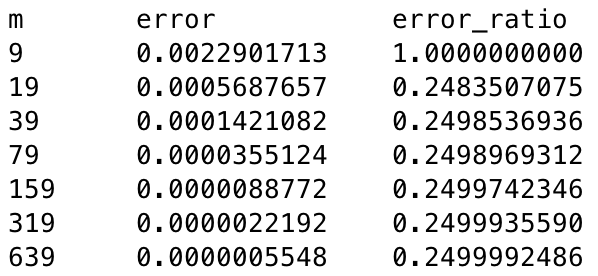
\includegraphics[width=2in]{q5out}
    \end{center}
    As $h$ halves, maximum error decreases by a factor of 4.
\end{proof}

 

\newpage
\section*{Appendix}
\section*{Problem 5 code}
\label{q5code}
\lstinputlisting[language=matlab]{code/q5.m}


\end{document}
